\section{Dreiphasen-Brückenschaltung - Gesteuerter Betrieb}

\begin{figure}[h!]
    \centering
    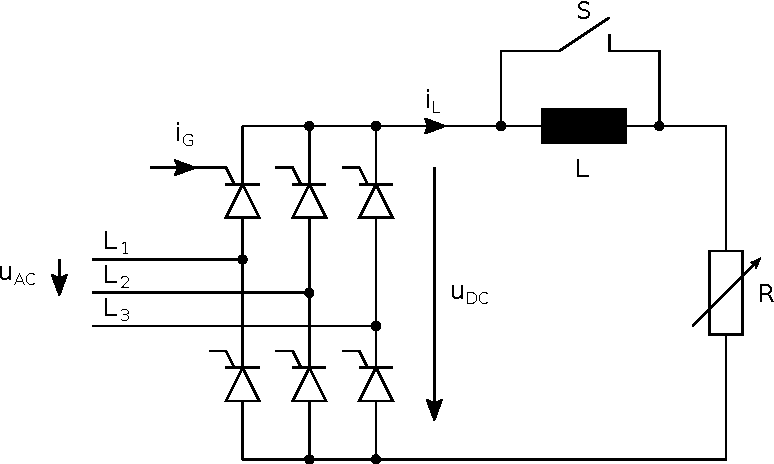
\includegraphics[scale=\sscale]{./../fig/b6_thyristor.pdf}
    \caption{B6 Thyristorgleichichter}
    \label{fig:b6_thyristor}
\end{figure}

\subsection{Messungen}

\begin{figure}[h!]
    \centering
    \includegraphics[scale=\pscale]{./../plots/642_01.pdf}
    \caption{B6 Thyristorgleichrichter mit L-Glättung}
\end{figure}

\begin{figure}[h!]
    \centering
    \includegraphics[scale=\pscale]{./../plots/642_02.pdf}
    \caption{B6 Thyristorgleichrichter mit L-Glättung}
\end{figure}

\begin{figure}[h!]
    \centering
    \includegraphics[scale=\pscale]{./../plots/642_03.pdf}
    \caption{B6 Thyristorgleichrichter mit L-Glättung}
\end{figure}

\begin{figure}[h!]
    \centering
    \includegraphics[scale=\pscale]{./../plots/642_04.pdf}
    \caption{B6 Thyristorgleichrichter mit L-Glättung}
\end{figure}

\begin{figure}[h!]
    \centering
    \includegraphics[scale=\pscale]{./../plots/642_05.pdf}
    \caption{B6 Thyristorgleichrichter mit L-Glättung}
\end{figure}

\begin{figure}[h!]
    \centering
    \includegraphics[scale=\pscale]{./../plots/642_06.pdf}
    \caption{B6 Thyristorgleichrichter mit L-Glättung}
\end{figure}

\clearpage
